%\documentclass[a4paper,french]{rnti}

\documentclass[a4paper,pagenum,french]{rnti}

\usepackage{graphicx}
\usepackage[T1]{fontenc}
\usepackage[utf8]{inputenc}
\usepackage{url}


\usepackage{amsmath,amsfonts,dsfont,amssymb,bm}
\usepackage{graphicx}
\usepackage[linesnumbered,ruled,vlined,french]{algorithm2e}
\usepackage{amsthm}
\usepackage{makeidx}
\usepackage{xcolor}
\usepackage{multicol}
\newtheorem{mydef}{Définition}
\theoremstyle{remark}
%\renewcommand{\emph}{\textbf}
\newenvironment{exemple}{%
\upshape Exemple: % Environnement quote
    \small     % ... en plus petit
}{%
}

% Titre court pour entête
\titrecourt{Prévention du risque de suicide grâce au Concept-drift}

\nomcourt{C. Maigrot et al.}

\titre{Prévention du risque de suicide dans les réseaux sociaux : Application de méthodes de Concept drift}

\auteur{Cédric Maigrot\affil{1},
        Sandra Bringay\affil{2}\affilsep\affil{3},
        Jérôme Azé\affil{2}}

\affiliation{
    \affil{1}IRISA Rennes, UMR 6074\\
    Cedric.Maigrot@irisa.fr\\
    %
    \affil{2}LIRMM, CNRS, UMR 5506\\
    \{Sandra.Bringay, Jerome.Aze\}@lirmm.fr\\
    %
    \affil{3}AMIS, Université de Montpellier Paul Valéry\\
    %
 }

\resume{%
Le suicide devient d'année en année une problématique plus préoccupante. Les organismes de santé tels que l'OMS se sont engagés à réduire le nombre de suicides de 10\% dans l'ensemble des pays d'ici 2020. 
Le suicide est souvent un geste impulsif cependant il existe souvent des comportements et des paroles qui peuvent révéler un mal être et représenter des signes précurseurs de prédispositions au suicide. L'objectif de cette étude est de mettre en place un système pour détecter semi-automatiquement ces comportements et ces paroles au travers des réseaux sociaux.
Des travaux précédents \cite{Abboute2014} ont proposé la classification de messages issus de Twitter suivant des thèmes liés au suicide : tristesse, blessures psychologiques, état mental,  etc. Dans cette étude, nous ajoutons la dimension temporelle pour prendre en compte l'évolution de l'état des personnes monitorées. Nous avons implémenté pour cela différentes méthodes d'apprentissage dont une méthode originale de \textit{concept drift}. Nous avons expérimenté avec succès sur des jeux de données réelles issues du réseau social Facebook.
%
}	

\summary{%
Suicide has long been a worrisome problem for society and is an event that has 
far-reaching effects.  Health organizations such as the World Health Organization (WHO) 
and the French National Observatory of Suicide (ONS) have pledged to reduce the 
number of suicides by 10\% in all countries by 2020.  While suicide is a very marked 
event, there are often behaviors and words that can act as early signs of predisposition to 
suicide.  The objective of this internship is to develop a system that semi-automatically 
detects these markers through social networks.  Previous work [1] has proposed the 
classification of Tweets using vocabulary in topics related to suicide: sadness, 
psychological injuries, mental state, depression, fear, loneliness, proposed suicide 
method, anorexia, insults, and cyber bullying.  
During this training period, we add a new dimension,  time to reflect changes in the status of monitored people. We implemented it with different learning methods including an original   \textit{concept drift} method. We have successfully experienced this method  on synthetic and real data sets issued from the  Facebook networks.
%
}


\begin{document}

%%%%%%%%%%%%%%%%%%%%%%%%%%%%%%
%%%%    chapitre INTRODUCTION  %%%%
%%%%%%%%%%%%%%%%%%%%%%%%%%%%%%
\section{Introduction}

Toutes les 40 secondes, une personne se suicide quelque part dans le monde\footnote{Prévention du suicide, L'état d'urgence mondial. OMS 2014. ISBN: 978 92 4 256477 8}. Toutes les régions et toutes les  tranches d’âge sont touchées, notamment  les jeunes âgés de 15 à 29 ans, pour qui le suicide est la deuxième cause de mortalité à l’échelle mondiale. Les méthodes proposées dans cette étude visent la prévention du suicide pour cette catégorie de personnes qui utilisent en majorité quotidiennement les réseaux sociaux. 
 
L'objectif de cette étude est de détecter les personnes à risques grâce aux messages laissés sur les réseaux sociaux (Twitter, Facebook, etc.).  Ce travail fait suite à la méthode décrite dans \cite{Abboute2014} qui permet d'associer à un message un niveau de risque. Dans cette étude, la méthode proposée se distingue en intégrant la dimension temporelle associée à l'évolution de l'état de la personne monitorée qui est capturée au travers de sa séquence de messages.

Nous avons adapté un modèle de \emph{concept drift} \cite{Gama2014} pour détecter ces changements d'états. L'idée est ici de  lever une alerte lorsque l'on détecte une évolution interprétée comme négative des messages au plus tôt mais sans solliciter abusivement le médecin qui sera le seul habilité à prendre la décision d'intervenir ou pas. 

Ce modèle intègre 3 modules : 
1) Prétraitement et mémorisation des messages avec notamment l'utilisation de différentes méthodes de Traitement Automatique de la Langue Naturelle (TALN) pour extraire des descripteurs pertinents des messages; 
2) Détection du niveau de risque des messages à partir d'une méthode ensembliste de classification (Stacking). 
3) Levée d'une alerte  à destination du psychiatre avec explication sur les raisons de la levée de l'alerte basée sur les résultats des étapes précédentes. La levée d'alerte est issue d'un calcul statistique sur la dérive d'un concept ou sur l'application de règles expertes	ou encore sur la comparaison de courbe ROC (\cite{hanley1982meaning}).

 Les challenges associés à ces travaux sont nombreux. Tout d'abord,  les méthodes de TALN doivent être adaptées pour traiter les données particulières issues des réseaux sociaux. %Les personnes ne maitrisant pas  l'orthographe et  la grammaire française lors de l'écriture des messages, les analyses syntaxico-sémantiques sont souvent faussées. 
 De plus, les techniques de \emph{concept drift} doivent  détecter des concepts  relativement subjectifs (\textit{e.g.}  anorexie,  dépression). \`A notre connaissance, il n'existe pas de ressources linguistiques comme des lexiques étoffés pour capturer ces concepts. 
 Les techniques doivent passer à l'échelle car le nombre de messages produits peut être très important. 
Le résultat du processus doit être clairement explicité au professionnel de santé afin de l'aider dans le processus de décision.
La mise à disposition des résultats des algorithmes de classification seuls n'est clairement pas suffisante.

Des études similaires ont déjà été réalisées (\textcolor{red}{REF}), cependant celle-ci se démarque à plusieurs niveaux. Tout d'abord, le travail réalisé se base sur les récits de personnes  ayant des comportements à risques avérés. Il s'agit de mails  transmis par l'Organisation Arrêt Demandé International \textit{OADI}\footnote{\url{http://oadi.education/}} travaillant sur les personnes harcellées et identifiées à risque par l'organisation et de messages récupérés sur les groupes Facebook traitant de thématiques à risque. Le processus mis en place prend en compte plusieurs niveaux de description : celui des concepts à risque évoqués dans un message (e.g. expression de la solitude, d'idéation suicidaire, récit de comportement anorexique, etc.), celui du niveau de risque défini selon le protocole de notre partenaire (l'association \textit{OADI}) et celui de l'alerte à transmettre ou non à l'équipe médicale chargée du monitoring.

 Les quatres contributions principales de cette étude sont : 1) la production d'une chaîne de traitements basée sur une technique de \textit{concept drift} qui prend en compte l'évolution des messages des personnes monitorées et non d'un seul message ; 2) la classification des messages selon 12 concepts, et 5 niveaux de risque en se basant  sur une méthode   ensembliste de classification (Stacking); 3) la constitution de lexiques spécialisés pour améliorer le premier niveau de description et l'utilisation d'un lexique de sentiments développé dans l'équipe; 4) des expérimentations sur des jeux de données réelles annotées manuellement.

Le reste de l'article est organisé comme suit. La section \ref{TravauxRelatifs} présente les travaux réalisés en lien avec notre étude. La section \ref{Methodes} présente la méthodologie mise en place. La section \ref{protocole} présente le protocole expérimental mit en place. Enfin, la section \ref{expe} présente les résultats obtenus.
%%%%%%%%%%%%%%%%%%
%%%%    chapitre Methodes  %%%%
%%%%%%%%%%%%%%%%%%

\section{\'Etat de l'art et motivations}\label{TravauxRelatifs}

\textbf{Fouille du web social pour des perspectives médicales.}
La santé est un domaine où la fouille des réseaux sociaux permet d’envisager de réelles perspectives médicales.  Depuis 2013, 2 milliards d'utilisateurs sont actifs dans ces réseaux sociaux. Facebook est le plus peuplé avec 1,2 milliards d’individus, suivi par d'autres réseaux, dont Twitter avec 225 millions. Ces réseaux sont très utilisés pour partager des pensées, opinions et émotions avec ses proches. Au cours des cinq dernières années, il y a eu un intérêt croissant pour exploiter ces réseaux  comme un outil pour la santé publique, par exemple pour analyser la propagation de la grippe \cite{Sadilek12modelingspread}. \cite{ICWSM112880}  utilisent des modèles thématiques pour capturer les symptômes et les traitements possibles pour des maux évoqués sur Twitter afin de définir des mesures de santé publique. En examinant manuellement un grand nombre de tweets, \cite{Krieck11anew} ont montré que les symptômes auto-déclarés sont le signal le plus fiable pour prévoir l'apparition d'une maladie. 
%Ces études utilisent généralement les fréquences de termes spécifiques (e.g. H1N1, grippe, fièvre) et elles manquent parfois des indices qui peuvent être trouvés par des méthodes syntaxiques et sémantiques.
%D’un point de vue médical, la qualité des solutions proposées et la fiabilité des résultats est difficile à estimer, surtout quand les conclusions sont fondées sur un échantillon restreint d'exemples triés sur le volet.

\textbf{Fouille du web social pour la détection des maladies mentales et des personnes suicidaires.}
Dans le cadre de cette étude, nous nous concentrons sur le potentiel des réseaux sociaux pour surveiller les populations à risque suicidaire.

D’autres recherches existent portant sur les  maladies mentales en général. Dans ces applications, une personne est considérée comme à risque selon son utilisation des médias sociaux. Par exemple, le contenu de leurs tweets, les mises à jour de leurs statuts Facebook, sont utilisés pour classer en temps réel les personnes selon des niveaux de risque.   \cite{citeulike:12521251}  a démontré que des mises à jour de statut sur Facebook révèlent des symptômes d'épisodes dépressifs majeurs. \cite{park2012} ont trouvé des preuves que les gens utilisent Twitter pour poster sur leur dépression et leur traitement. Tous ces travaux soulignent le potentiel des médias sociaux comme une source de signaux pour la maladie mentale. 
Plus précisément, autour de la thématique du suicide, \cite{CashTPFB13}  analysent les messages d’adolescents sur MySpace.com afin de déterminer les sujets à risque (relations, santé mentale, toxicomanie/abus, méthode de suicide, déclarations sans contexte). \cite{Jashinsky14}  étudient les facteurs de risque de suicide par Twitter et trouve une forte corrélation entre les données Twitter dérivées et les données sur le suicide, ajustés selon l'âge. \cite{HomanSS13}  se concentrent sur un aspect particulier des tendances suicidaires, la détresse qui est un facteur de risque important dans le suicide et qui est observable à partir des textes de microblogs. Ils extraient des sujets d'intérêt pour les personnes à risque avec des techniques de modélisation non supervisées et ils mettent en place des méthodes de classification automatique pour identifier les personnes en détresse. \cite{Christensen} soulignent que des interventions sont possibles, bien que la validité, la faisabilité et la mise en œuvre reste incertaine car peu d'études ont été menées à ce jour dans des conditions réelles.

%Nous nous concentrons sur des données correspondant à des récits issus du réseau social Facebook et des données fournies par une association partenaire \textit{OADI} pour modéliser des concepts liés au suicide, différents niveaux de risque et un protocole de levée d'alerte. 
%L'originalité de notre approche est de prendre en compte non seulement les aspects thématiques mais également leur évolution temporelle via une adaptation d'un protocole de \textit{concept drift}. Nous invitons le lecteur a se reporter au document d'état de l'art (rédigé en avril) pour une bibliographie sur les méthodes de \textit{concept drift}.
%=====
%===== SECTION "Architecture du projet" =====
%=====
\section{Processus global de surveillance des individus}\label{Methodes}


Le processus  de surveillance des patients est inspiré globalement des méthodes de \textit{concept drift} qui permettent de capturer l'apparition de nouveaux concepts au cours du temps. Nous avons repris l'architecture de \cite{Gama2014} que nous avons modifié pour intégrer le fait que nous ne connaissons pas la véritable nature des données (niveau de risque à prédire) sans intervention du professionnel de santé et pour intégrer des règles expertes pour la levée d'alerte. 

Le processus est organisé  en  $3$ modules indépendants décrit comme suit :
1) la mémorisation et le prétraitement des messages (voir Section \ref{module1});
2) la détection du niveau de risque associé à un message (voir Section \ref{module2});
3) la levée d'alerte (voir Section \ref{module3}).

Les deux premiers modules font une analyse individuelle des messages, le troisième récupère alors les messages d'un même utilisateur afin de les comparer pour lever ou non une alerte.

%*** SUBSECTION "Module de mémorisation des données" ***
\subsection{Module 1 : mémorisation des messages et prétraitements}\label{module1}

L'objectif de ce module est de mémoriser pour chaque personne monitorée :
%La mémorisation des messages est nécessaire car lors de la classification d'un message, les anciens messages du même auteur peuvent avoir de l'importance. Ainsi, lors de la réception d'un nouveau message, il faut être capable de déterminer le niveau de risque des anciens messages.
%Lors de la mémorisation des exemples, le module mémorise toutes les informations liées à l'exemple :
\begin{itemize}
\item le groupe Facebook auquel elle appartient ainsi que la thématique du groupe (e.g. tentative de suicide, harcèlement, anorexie, etc);
\item le contenu de ses messages,  la date et l'heure de l'écriture des messages, le nombre de mentions \emph{likes}, le nombre de commentaires;
\item les commentaires associés à un message;
\end{itemize}

Il est important de noter que cette démarche est aussi applicable à de nombreux autres réseaux sociaux (e.g Twitter, Instagram, Ask... ).

Comme indiqué par \cite{Balahur2013}, les textes issus des réseaux sociaux ont des particularités linguistiques qui peuvent influencer les performances de la classification. Pour cette raison nous avons appliqué les prétraitements suivants :
1) remplacement des noms d'utilisateurs par [NOM];
2) remplacement des adresses mails par [MAIL];
3) remplacement des adresses URL par [URL];
4) remplacement des émoticônes par un mot d'humeur associé (table de correspondance créée pour l'étude);
5) remplacement des abréviations par le(s) mot(s) complet(s) (table de correspondance créée pour l'étude);
6) suppression des accents et des majuscules, en effet certaines personnes n'utilisent pas ces deux conventions d'écritures sur les réseaux sociaux afin d'écrire plus vite. Leur normalisation en minuscules sans accent permet alors de restreindre le nombre de N-Grammes générés et ainsi faire le lien entre des messages ne présentant par avant aucun N-Grammes;
7) lemmatisation de tous les mots en utilisant l’outil TreeTagger (\cite{Schmid1994}).
%*** SUBSECTION "Module d'apprentissage" ***
\subsection{Module 2 : détection du niveau de risque en 2 étapes}\label{module2}

Le module de détection du niveau de risque se déroule en 2 étapes.
Nous avons choisi de travailler en respectant le paradigme de l’ensemble learning qui consiste à apprendre plusieurs classifieurs dans le but de résoudre le même problème.
%Les premiers travaux consacrés à l’ensemble learning datent des années 1990  (\textbf{\cite{Hancock1990, Wolpert1992, Krogh1995, Aze2012}}). Par opposition à l’apprentissage “classique” où un seul classifieur est appris, l’ensemble learning apprend un ensemble de classifieurs qui sont ensuite combinés pour obtenir un méta-classifieur. 

Nous nous sommes placés dans ce paradigme pour les quatre raisons suivantes : 1) la combinaison de classifieurs donne en général de meilleurs résultats (\cite{wang2003mining}); 2) la puissance de calcul à notre disposition rend accessible l’apprentissage et l’utilisation de nombreux modèles pour résoudre le même problème ; 3) les  masses de données à traiter  pourraient s’avèrer  non apprenables par un unique classifieur;
4) le besoin d'expliciter les résultats de la classification pour les humains impliqués dans le processus de prise de décision. %Nous reviendrons sur ces trois éléments lors de l'évaluation de notre méthode.

Diverses formes d’ensemble learning peuvent être citées : \emph{Stacking}, \emph{Boosting} et \emph{Bagging}. 
%Elles divergent principalement par la fonction d’aggrégation mise en œuvre pour obtenir le méta-classifieur. Ces divergences peuvent avoir un impact sur l’apprentissage : modification des exemples pendant l’apprentissage (Stacking), modification de l’importance relative des exemples (Boosting); ou uniquement en post-traitement de l’apprentissage pour combiner les différents modèles appris (Bagging).
Dans notre contexte, nous avons choisi l'approche \emph{Stacking} qui consiste à apprendre une succession de classifieurs organisés en  deux niveaux et aggrégés selon un vote majoritaire et tels que chaque classifieur apprenne de nouveaux descripteurs permettant de redécrire les données.

Nous détaillons dans la suite ces deux étapes dans les sections  \ref{etape1} et  \ref{etape2}.

\subsubsection{Première étape : détection des concepts dans un message}\label{etape1}

La première étape permet de repérer dans les messages un premier niveau d'information :   la présence ou l'absence d'un signal de mal-être que nous nommerons par la suite \emph{concept}. La liste des \emph{concepts} considérés est: \emph{précédente tentative de suicide}, \emph{idéations suicidaires}, \emph{dépression}, \emph{harcèlement}, \emph{prise aux médicaments}, \emph{problème d'alimentation} (anorexie ou boulimie), \emph{auto-mutilation}, \emph{colère}, \emph{peur}, \emph{solitude}, \emph{tristesse} et  \emph{rémission}. Cette liste issue des travaux de \cite{Plutchik1994} a été validée par des experts psychiatres. Pour chaque concept, un classifieur renvoie la valeur \emph{oui} ou \emph{non} pour associer la présence ou l'absence du concept dans le message. 
Nous avons choisi  les descripteurs résumés ci-dessous que nous avons complétés avec des lexiques spécifiques pour chaque concept. 

%\section{Caractéristiques utilisées} \label{caracteristiques}
%*** SUBSECTION "Caractéristiques provenant de Facebook" ***
%\subsection{Caractéristiques provenant de Facebook}
%Plusieurs informations pouvant déterminer le niveau de risque d'un exemple proviennent directement de Facebook. Leur prise en compte est donc indispensables à une bonne classification : 
\begin{itemize}

\item Contenu du message décrit par les mesures statistiques suivantes : 1) un ensemble de N-grammes pour permettre une comparaison entre les messages sélectionnés selon la mesure \emph{TF-IDF} pour ne conserver que les mots discriminants par concepts ; % \textbf{Moins qu'à son habitude}\\ 
%2)  la présence d'élément subjectifs dans la phrase : nous avons réutilisé la chaîne de traitements produite dans l'équipe \cite{Abdaoui2015} qui classe les phrases dans les catégories \textit{information}  (e.g. partage d'un lien relatant une histoire de harcèlement) ou \textit{subjective} (e.g.  confidence de la victime sur un harcèlement subit plus tôt dans la journée);
%3) le nombre de mots de polarité(s) (\textit{négatif, positif ou neutre}) et d'émotion(s) (\textit{joie, colère, etc.}) : l'apparition des sentiments dans les récits est fréquent voir omni-présente. La \emph{peur} est le sentiment le plus  souvent rencontré avec la \emph{tristesse} et la \emph{colère} (voir annexe \ref{annexe_sentiments}). Nous avons utilisé le lexique \cite{Abdaoui2014} produit dans l'équipe et décrit dans l'annexe \ref{annexe_feel} ; 
%\item    Polarité des commentaires d'un exemple & Pour compléter l'orientation d'un message, la mesure définissant la polarité majoritaire des commentaires est définie. La polarité peut est positive, négative ou neutre. Pour cela, on utilise un module externe réalisé au sein de l'équipe [REF]\textbf{Ref Amine et Mike}.\\
 %La notion d'estimation du niveau de risque ne porte que sur le second cas car seul ce type de message décrit l'état de la victime. Il est donc intéressant de pouvoir repérer les messages n'apportant qu'une information.
2) le nombre de mots associés à un concept donné par un lexique réalisé pour l'étude.
\item Nombre de commentaires : un message à risque est suceptible de soulever beaucoup de réactions auprès des autres membres du groupe ;
\item Nombre de mentions \emph{Likes} : à l'inverse, un message où la victime évoque son bien-être ou son rétablissement peut être accompagné de beaucoup de mentions \emph{Likes} ;
\item Longueur du message : deux comportements opposés des victimes sont connus \textcolor{red}{REF}. La victime peut écrire des messages plus longs par besoin de se confier aux autres ou au contraire se refermer sur elle-même et moins écrire;

%\item    Niveau de risque des messages précédents : %le passé de la victime est important  car une personne étant déjà passée à l'acte est plus susceptible de recommencer.  
%Si les exemples précédents ont un haut niveau de risque, un risque de passage à l'acte est plus plausible. Pour calculer la valeur de cette caractéristique, la moyenne du niveau des anciens messages est calculé mais d'autres approches pourraient être testées (e.g. nombre de messages de chaque niveau).
\end{itemize}



En sortie de cette étape, un message est associé à un vecteur de concepts dans lesquels on stocke un booléen.
Par exemple, le message "\textit{Je vais tres mal, aidez moi vite svp. Je me fais harcelee depuis 3ans et me fais frapper tous les jours. Je mappelle lea, jai 14ans et vis a roubaix}" est associé au vecteur 
(
$\overline{\mbox{\emph{tentative de suicide}}}$, 
$\overline{\mbox{\emph{idéations suicidaires}}}$,
$\overline{\mbox{\emph{dépression}}}$,
\emph{harcèlement},
$\overline{\mbox{\emph{médicaments}}}$,
$\overline{\mbox{\emph{anorexie}}}$,
$\overline{\mbox{\emph{mutilation}}}$,
$\overline{\mbox{\emph{colère}}}$,
\emph{peur},
$\overline{\mbox{\emph{solitude}}}$,
\emph{tristesse},
$\overline{\mbox{\emph{rémission}}}$
).

%\paragraph{Présence d'un élément complémentaire au message (lien, photo, etc. )} : Certaines personnes postent une photo pour accompagner 


%*** SUBSECTION "Caractéristiques calculés" ***
%\subsection{Caractéristiques calculées} 
%Afin de compléter la liste des caractéristiques définissant un exemple, d'autres caractéristiques sont calculées en se basant sur les caractéristiques précédemment citées.


\subsubsection{Deuxième étape : calcul du niveau de risque pour un message}\label{etape2}

La seconde étape utilise les sorties de la première étape comme descripteurs pour prédire le niveau de risque des messages. Les niveaux de risque sont répartis sur cinq niveaux représentant les messages non à risque (niveau 0), présentant un ancien risque (niveau 1), à risque faible (niveau 2), à risque modéré (niveau 3), à risque élevé (niveau 4).

Les $5$ niveaux de risque en sortie étant difficiles à interpréter en terme de levée d'alerte, nous avons simplifié le problème en prédisant $2$ niveaux de risque après regroupement des niveaux 0 et en \textit{risque faible} ainsi que 2, 3 et 4 en \textit{risque élevé}.
%*** SUBSECTION "Module d'estimation des pertes" ***
\subsection{Module 3 : levée d'une alerte}\label{module3}

Pour la levée d'une alerte, nous avons décidé de comparer 3 modèles : 1) un modèle de dérive des concepts via l'estimation classique des pertes  en \textit{concept drift} (voir  section  \ref{pertes}); 2) un modèle par comparaison de courbe ROC (voir  section \ref{roc}); 3)  un modèle basé sur des règles expertes telles que fournies par l'association partenaire (voir  section  \ref{regles}).

\subsubsection{Modèle basé sur l'estimation des pertes}\label{pertes}

La plupart des algorithmes de \emph{concept drift} \cite{Gama2014} considèrent des tâches pour lesquelles on connait, à un certain moment, la vraie valeur associée aux données à prédire. Par exemple, pour des relevés de températures, on peut prédire des valeurs puis mesurer la vraie valeur que l'on peut comparer aux prévisions pour estimer les pertes, c'est-à-dire l'écart entre la prédiction et la vérité et lever une alerte si les pertes sont trop élevées (i.e les prédictions sont trop souvent fausses). Dans notre cas, la "vérité" n'est pas disponible sans intervention du professionnel de santé que l'on souhaite minimiser. Nous avons donc adapté le calcul réalisé par \cite{Bach2010} pour estimer les pertes à un instant donné en considérant le taux d'accord entre les classifieurs (i.e on compte le nombre de classifieurs ayant réalisé la même prédiction).

Soit une fenêtre $\mathcal{F}$ glissante contenant les $N$ derniers exemples de l'utilisateur (lors de l'arrivée d'un nouveau message, le plus ancien est supprimé). Le $1^{er}$ et le $N^e$ exemples décrivent respectivement le message le plus ancien et le plus récent.
Le taux d'erreur $\delta$ au temps $t$, noté $\delta_t$ est donné par :
\[
\delta_t = \frac{\sum\limits_{i=1}^N bienClasse(i)}{N}
\]

où $bienClasse(i)$ retourne le taux d'accord de la prédiction retenue (i.e le nombre de classifieurs ayant prédit le niveau retenu sur le nombre de classifieurs). 

Cependant, il est important de pondérer l'instant dans le temps d'une erreur de classement. Pour cela, un système d'\emph{oubli progressif} (\cite{Chandramouli}) est mis en place. Ainsi, chaque erreur est coefficientée selon son ancienneté :
\[
\delta_t = \frac{\sum\limits_{i=1}^N (bienClasse(i)*\frac{i}{N})}{\frac{N+1}{2}}
\]

Les $N$ dernières valeurs $\delta$ sont mémorisées, soit le $\delta$ associé à chacun des $N$ messages précédemment nommés. 
Une alerte est levée si la moyenne des $N$ $\delta$ dépasse un seuil $\Delta$ fixé par l'utilisateur. Si c'est le cas, l'ensemble des $N$ valeurs $\delta$ sont transmises au module de détection de changement pour calculer le temps pour lequel le changement a eu lieu et lancer une procédure d'alerte auprès du psychiatre référent. 

Pour l'interprétation du professionnel de santé, il est important de lui pointer le temps où un concept est apparu pour l'aider dans son analyse.
Si une dérive du modèle est constatée, il faut réapprendre un nouveau modèle à partir de ce moment. Pour cela, on cherche $\Omega$ tel que :
\begin{itemize} 
\item $\Omega$ soit l'indice de l'exemple parmi l'ensemble des $N$ exemples. Soit $1 \leq \Omega \leq N$;
\item La différence des moyennes des valeurs d'estimation des pertes des sous-ensembles définit par les bornes $[1,\Omega-1]$ et $[\Omega,N]$ soit maximale.
\end{itemize}

Ainsi, l'algorithme~\ref{algo:cd}, que nous proposons, donne le temps $t$ où le changement de concept est le plus plausible. Afin de déterminer au mieux l'instant du changement de comportement.

\begin{algorithm}
\DontPrintSemicolon
\Donnees{Une fenêtre glissante $\mathcal{F}=\{\delta_1, \delta_2, \ldots, \delta_N\}$ de valeurs numériques}
\Res{L'indice $\Omega$ qui maximise l'écart de moyenne entre les sous-ensembles $\mathcal{F}_1$ et $\mathcal{F}_2$ bornés respectivement par $[1,\Omega-1]$ et $[\Omega,N]$}
$\Omega \gets 1$\;
$diff_\Omega \gets 0$\;
\Pour{$i \gets 2$ \textbf{à} $N$} {
	$somme_1 \gets 0$\;
	\Pour{$j \gets 1$ \textbf{à} $i-1$} {
    	$somme_1 = somme_1+ \mathcal{F}_{j}$\;
    }
    $moyenne_1 \gets \frac{somme_1}{i-1}$\;
    
    $somme_2 \gets 0$\;
	\Pour{$j \gets i$ \textbf{à} $N$} {
    	$somme_2 = somme_2+ \mathcal{F}_{j}$\;
    }
    $moyenne_2 \gets \frac{somme_2}{(N-i)+1}$\;
  \Si{$diff_\Omega < |moyenne_1-moyenne_2|$} {
    $\Omega = i$\;
    $diff_\Omega = |moyenne_1-moyenne_2|$\;
  }
}
\Retour{$\Omega$}\;
\caption{{\bsc{Detection du temps de Changement}}}
\label{algo:cd}
\end{algorithm}
\subsubsection{Modèle basé sur la comparaison de courbe ROC}\label{roc}

% Nous avons ici reformuler le problème pour lever une alerte quand on trouve au moins un message posté par l'utilisateur  tel que le niveau de risque associé à ce message soit élevé. Pour atteindre cet objectif, plusieurs approches peuvent être mise en \oe uvre : apprentissage de classifieurs pour le niveau de risque (classification), apprentissage d'une fonction permettant d'associer un risque à chaque message (régression) ou encore apprentissage d'une fonction permettant d'ordonner les messages par risque croissant.

% L'approche que nous allons présenter ici relève de ce dernier cas d'utilisation.
% Nous allons utiliser l'algorithme ROGER (ROc based Genetic learnER) initialement proposé en 2003 dans le cadre de la prédiction du risque cardio-vasculaire \cite{SebagAzeLucas:ICDM2003,SebagLucasAze:EA2003,Challenge_PKDD03}.
% Cet algorithme a été adapté et utilisé avec succès dans plusieurs autres cadres applicatifs : l'extraction de la terminologie \cite{Aze_ROCML:2005}, de la prédiction d'interactions entre protéines \cite{deVienne-Aze_PLoSOne:2012} ou encore de la prédiction de complexes protéines-protéines \cite{PLoSOne:2011}.

% L'algorithme ROGER apprend des fonctions de la forme : $f({\bm x_i}) = \sum_j w_j \times {\bm x_i}(j)$ où ${\bm x_i}(j)$ représente la valeur de la  $j^{ème}$ composante de l'exemple ${\bm x_i}$.
% L'algorithme apprend les poids $w_j$ tels que $\sum_i rang_f({\bm x_i}) \times \mathds{1}_{y_i = +1}$ soit minimale (où $rang_f({\bm x_i})$ correspond au rang de l'exemple ${\bm x_i}$ induit par la fonction $f$, et $\mathds{1}_{y_i = +1}$ correspondant à la fonction indicatrice qui vaut 1 si la classe de ${\bm x_i}$ est positive et 0 sinon).

% Il est aisé de montrer qu'une fonction maximisant l'aire sous la courbe ROC minimise la somme des rangs des exemples positifs qu'elle ordonne.

La  \textbf{courbe ROC} (Receiver Operating Characteristic) \cite{RocLift:2006,ROC:1978} représente un classifieur ayant la capacité de séparer parfaitement les positifs des négatifs.

Nous allons utiliser l'algorithme ROGER (ROc based Genetic learnER) initialement proposé en 2003 dans le cadre de la prédiction du risque cardio-vasculaire \cite{SebagAzeLucas:ICDM2003,SebagLucasAze:EA2003,Challenge_PKDD03}. Cet algorithme a été adapté et utilisé avec succès dans plusieurs autres cadres applicatifs : l'extraction de la terminologie \cite{Aze_ROCML:2005}, de la prédiction d'interactions entre protéines \cite{deVienne-Aze_PLoSOne:2012} ou encore de la prédiction de complexes protéines-protéines \cite{PLoSOne:2011}.

L'algorithme ROGER apprend des fonctions de la forme : $f({\bm x_i}) = \sum_j w_j \times {\bm x_i}(j)$ où ${\bm x_i}(j)$ représente la valeur de la  $j^{ème}$ composante de l'exemple ${\bm x_i}$.
L'algorithme apprend les poids $w_j$ tels que $\sum_i rang_f({\bm x_i}) \times \mathds{1}_{y_i = +1}$ soit minimale (où $rang_f({\bm x_i})$ correspond au rang de l'exemple ${\bm x_i}$ induit par la fonction $f$, et $\mathds{1}_{y_i = +1}$ correspondant à la fonction indicatrice qui vaut 1 si la classe de ${\bm x_i}$ est positive et 0 sinon).


Dans notre contexte, ROGER permet d'apprendre à ordonner les messages des utilisateurs par risque décroissant.
Sous l'hypothèse qu'il existe au moins un \textit{concept drift} par utilisateur, nous considérons que le message le plus à risque (prédit par ROGER) est le message correspondant au drift.
\subsubsection{Modèle basé sur les règles expertes}\label{regles}

%La troisième couche consiste à classer l'instance en deux classes (\textit{alerte} et \textit{non alerte}) selon des règles expertes.  
%Comme il n'est pas possible de compter en permanence sur la participation du professionnel pour étiquer les messages et calculer l'estimation des pertes, 
Nous avons également implémenté des règles expertes fournies par l'association \textit{OADI} pour la levée de l'alerte et nous avons exploré les scénarios suivants. Une alerte est levée si il y a : 
1) un message avec un risque  de niveau 4 dans les $N$ derniers messages;
2)  une augmentation du niveau de risque entre 2 temps consécutifs;
3)  une augmentation du niveau de risque avec un écart de au moins 2 niveaux sur une fenêtre de $N$ messages; Nous ferons varier $N$ pour évaluer les performances pour détecter des changements abrupts ou lents;
4)  des oscillations du niveau de risque.

On obtient alors les règles suivantes : Soit $M$ l'ensemble des $N$ derniers messages d'un utilisateur où $M_1$ correspond au message le plus ancien et $M_N$ au plus récent. On notera $R_i$ le niveau de risque du message $i$.

% * <jeromeaze@gmail.com> 2015-09-21T10:03:18.541Z:
%
%  Dans le contexte, je ne comprend pas 
%
\begin{itemize}
\item  $\exists i, 0\leq i \leq N | R_i = 4$
\item  $\exists i, 0\leq i \leq N-1 | R_i < R_{i+1}$
\item  $\exists i, 0\leq i \leq N-1 | R_i < (R_{i+1}-1)$
\item  $\exists i \exists j, 0\leq i \leq N-1, 0\leq j \leq N-1 | R_i < R_{i+1}, R_j > (R_{j+1})$
\end{itemize}

\begin{figure}[!h]
   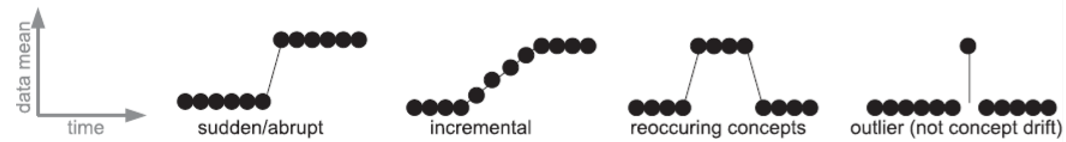
\includegraphics[width=.95\textwidth]{imgs/types_concept_drift.png}
	\caption{\label{formes_cd} Les différentes formes de \emph{concept drift} (adaptés de \cite{Gama2014})}
\end{figure}

Le schéma \ref{formes_cd} représente les différentes formes de changement que nous souhaitons capturer via les règles expertes : 
1) Le changement \emph{immédiat} correspond à un individu qui parle du jour au lendemain de méthode de suicide;
2) Le changement \emph{incrémental} correspond au cas où l'individu parle de plus en plus de son mal être;
3) Le changement \emph{récurrent} est un utilisateur qui régulièrement parle de son mal être;
4) Le \emph{bruit} serait un message isolé parlant de suicide.

%En sortie de ce module, quelque soit les variantes implémentées, nous obtenons la levée ou non d'une alerte pour un individus, le message ayant sucité la levée de l'alerte, les annotations en terme de concept et de risque (issue du module 2) qui vont aider le professionnel de santé à prendre la décision d'intervenir ou non.
%%%%%%%%%%%%%%%%%%%%%%%
%%   chapitre PROTOCOL EXPERIMENTAL
%%%%%%%%%%%%%%%%%%%%%%%
\section{Protocol expérimental}\label{protocole}

L'objectif de ces expérimentations est double.
% Tout d'abord nous nous sommes assurés du bon fonctionnement de l'algorithme de \emph{concept drift} sur un jeu synthétique de la littérature (SEA, \cite{Street2001}) pour évaluer ses performances pour différentes types de dérives (travaux non présentés dans cet article par manque de place). Nous avons ensuite expérimenté sur un jeu de données réelles, en récupérant des messages issus de groupes de paroles à risque de Facebook et de mails fournis par l'association  \textit{OADI}.


\subsection{Données utilisées}
Cette étude a porté sur l'analyse de messages écrits par des populations à risque. Pour cela, nous avons commencé par utiliser des messages fournis par l'association \textit{OADI} qui travaille avec des victimes de harcellement. Nous nous sommes ensuite intéressé à des messages directements issus de groupes Facebook que nous avons récoltés via l'API Facebook\footnote{http://developers.facebook.com}.

Nous avons sélectionné plusieurs groupes ayant pour thématique un ou plusieurs facteurs de risque connus pour le suicide (\emph{suicide}, \emph{anorexie}, \emph{mutilation} ou \emph{harcèlement}). Les auteurs sont généralement des adolescents entre $13$ et $18$ ans. Il est important de noter que ces groupes comprennent aussi des adultes dans la situation d'anciennes victimes  qui viennent témoigner de leur expérience dans ces groupes. Il est aussi possible de trouver des messages de parents ou de proches qui viennent demander des conseils pour leur enfant possiblement harcelé. Nous avons récolté 4597 messages entre le 15 Mars 2015 et le 3 Juin 2015.

Dans le cadre de nos expérimentations, nous avons sélectionné manuellement 22 comptes ayant entre 3 et 14 messages postés sur les groupes. Ils respectent les conditions suivantes : 1) L'auteur est une personne à risque; 2) La personne évoque son bien/mal-être; 3) La personne n'est pas un modérateur du groupe (les messages d'administrations pouvant fausser l'analyse). Nous avons alors obtenu 141 messages.

L'association \emph{OADI} %\footnote{Organisme Arret Demandé Internatial, http://oadi.education/} qui est un organisme d'aide aux personnes harcelées. Les messages sont accompagnées d'un niveau de risque estimé par le personnel de l'organisme. L'organisme utilise un système à $4$ niveaux : 
nous a également fourni un protocole utilisé par les volontaires pour détecter le niveau d'urgence. Nous l'avons adapté à notre cas d'étude qui ne se limite pas au cas des personnes harcellées. Nous considérons 5 degrés d'urgence :1) \emph{Pas d'urgence} : Il n'y a aucune urgence à traiter le message de la personne;
2) \emph{Risque minimal} : Le problème de la personne se situe dans le passé. Cette situation  est encore difficilement supportable pour la personne, elle estime que sa parole doit être libérée;
3) \emph{Risque intermédiaire} : La personne a un problème. L'isolement commence à s'installer;
4) \emph{Risque important} :  La personne a un problème durable pouvant inclure de la violence. Un isolement important s'installe;
5) \emph{Risque absolu} : La personne est violente verbalement et/ou physiquement. Elle tient des propos suicidaires et/ou se met en danger elle-même.

Les 168 messages ont été annotés manuellement par trois personnes. Chaque message a reçu au total 13 annotations : présence ou abscence des 12 concepts et un niveau de risque. Le kappa de Fleiss donne une valeur de 0,563 pour les cinq niveaux de risque.

\subsection{Évaluations}
\subsubsection{Détection du niveau de risque}
Lors de l'étape 1 du module 2 pour détecter les concepts dans un message, nous avons souhaité favoriser une bonne classification des messages possédant un concept. %afin de ne jamais sous-estimé la gravité d'un message. 
L'objectif est de trouver la meilleure configuration qui maximise le \emph{rappel} de la classe \emph{oui} (i.e minimiser le nombre de messages devant être classés comme \emph{"oui"} et qui sont classés comme \emph{"non"}). De la même manière, le classifieur utilisé pour le $2^e$ niveau doit être capable de maximiser le \emph{rappel} de la classe de plus haut niveau (i.e niveau 4 dans le cas d'une classification sur 5 classes et niveau 1 dans le cas d'une classification binaire du niveau de risque). Il est important de bien classer un message présentant un haut niveau de risque pour être sûr de réagir à un tel message. Afin de réaliser le principe d'ensemble learning, cinq classifieurs  (\emph{J48}, \emph{JRip}, \emph{SMO}, \emph{Naive Bayes}, \emph{IB1}) sont utilisés pour chaque prédiction grâce à l'outil Weka \cite{hall2009weka}. La validation est effectuée par validation croisée en mode Leave-one-out.

\subsubsection{Levée d'une alerte}

La levée d'alerte doit traiter les messages d'un utilisateur en même temps. Pour cela, l'intégralité des messages associé à un niveau de risque est transmis au module 3. On admet que chaque utilisateur à présenté un risque (i.e. une alerte doit être levé dans la séquence de messages). Pour cela, nous imposerons que le message correspondant à l'instant de la levée d'alerte ne peut être le premier message posté n'ayant aucune indication de l'état "normal" de la personnes à cet instant précis. De plus, dans le cas où plus messages seraient qualifiable de \emph{message le plus à risque}, le plus ancien est retenu afin de réagir le plus vite possible à un risque de passage à l'acte.


\paragraph{Estimation des pertes : } L'estimation des pertes est évalué grâce au calculs présentés dans la partie précédente.

\paragraph{ROGER : } L'algorithme présente directement, de part les scores attribués aux messages, le message le plus probable d'être à risque.

\paragraph{Règles expertes : } Chaqu'une des $4$ règles est testée sur chaque message. Le message ayant répondu positivement au maximun de règle est qualifié de message le plus à risque.
%%%%%%%%%%%%%%%%%%%%%%%%%%%%%
%%%%%%%%%%%%%%%%%%%%%%%%%%%%%
\section{Expérimentations sur des données réelles}\label{expe}

\subsection{Détection du niveau de risque ($1^{ere}$ étape)}

Cette première couche de détection, qui utilise les informations provenant de Facebook ainsi que les résultats des prétraitements, détermine la présence ou non des $12$ concepts. Par manque de place, nous présentons les résultats des concepts \emph{Harcèlement},\emph{Peur} et \emph{Solitude}.
La première constation est que chaque classifieur s'adapte différement selon les concepts (e.g. \emph{Naive Bayes} est efficace sur la détection du harcèlement, alors que la peur et la solitude sont mieux captés par l'algorithme \emph{J48}). 

\begin{table}[htb]
\center\small
\begin{tabular*}{\linewidth}{@{\extracolsep{\fill}}lccc}
\hline\hline
& Harcèlement & Peur & Solitude\\
\hline
J48
& 47,1\% \footnotesize{(64,8\%)} &  \textbf{60,0\% \footnotesize{(89,6\%)}} &  \textbf{61,5\% \footnotesize{(86,1\%)}} \\
Naive Bayes
& \textbf{54,9\% \footnotesize{(70,0\%)}} & 52,0\% \footnotesize{(82,4\%)} & 53,8\% \footnotesize{(88,2\%)} \\
IB1
& 05,8\% \footnotesize{(59,1\%)} & 24,0\% \footnotesize{(82,0\%)} & 30,8\% \footnotesize{(82,5\%)} \\
JRip
& 27,5\% \footnotesize{(62,0\%)} & 40,0\% \footnotesize{(84,0\%)} & 53,8\% \footnotesize{(88,7\%)} \\
SMO 
& 37,3\% \footnotesize{(70,2\%)} & 56,0\% \footnotesize{(90,5\%)} & 34,6\% \footnotesize{(83,8\%)} \\
Vote 
& 29,4\% \footnotesize{(69,8\%)} & 48,0\% \footnotesize{(88,9\%)} & 46,2\% \footnotesize{(86,7\%)} \\
\hline
\end{tabular*}
\caption{Résultat des classifieurs sur la détection du harcèlement, de la peur et de la solitude}
\label{tab_precision_concept}
\end{table}

\subsection{Détection du niveau de risque ($2^{eme}$ étape)}

Les six classifieurs sont ensuite appliqués à la seconde couche de prédiction (prédiction du niveau de risque). Pour cela, 4 tests sont réalisés : une prédiction binaire et une prédiction en cinq niveaux de risque dans le cas d'une prédiction à partir des concepts et dans le cas d'une classification directement à partir des messages Facebook. Le tableau \ref{tab_precision_niveau} présente ces résultats par les deux mesures retenues pour différencier les classifieurs : en premier le rappel sur le niveau le plus à risque, et en cas d'égalité la F-Mesure globale (entre parenthèse dans le tableau). Une première constatation non surprenante est que la classification binaire obtient de meilleures résultats que la classification en 5 niveaux de risque. De plus, on remarque que notre choix de modèle Stacking obtient de meilleures résultats que la prédiction directe depuis les messages Facebook. En effet, certains classifieurs obtiennent un rappel très élevé sur ce test (e.g. IB1 pour la prédiction directe en cinq niveaux de risque) mais cela est obtenu en classant une grande majorité des messages dans la classe de niveau le plus élevé, ce qui ne se révèle pas efficace en réalité comme le montre le score de F-Mesure associé (e.g. 6,6 \%)

\begin{table}[htb]
\center\small
\begin{tabular*}{\linewidth}{@{\extracolsep{\fill}}lcccc}
\hline\hline
& 2 niveaux (Stacking) & 5 niveaux (Stacking) & 2 niveaux (Direct) & 5 niveaux (Direct) \\
\hline
J48
& 92,6\% \footnotesize{(89,2\%)} & 83,3\% \footnotesize{(59,2\%)} 
& 70,4\% \footnotesize{(57,8\%)} & 23,3\% \footnotesize{(25,5\%)}\\
Naive Bayes
& 88,9\% \footnotesize{(85,7\%)} & 73,3\% \footnotesize{(44,5\%)} 
& \textbf{99,1\% \footnotesize{(50,0\%)}} & 26,7\% \footnotesize{(29,8\%)}\\
IB1
& 88,0\% \footnotesize{(80,1\%)} & 73,3\% \footnotesize{(50,1\%)} 
& 47,2\% \footnotesize{(53,2\%)} & \textbf{96,7\% \footnotesize{(06,6\%)}}\\
JRip
& 92,6\% \footnotesize{(92,6\%)} & \textbf{83,3\% \footnotesize{(92,6\%)}} 
& 70,4\% \footnotesize{(92,6\%)} & 23,3\% \footnotesize{(92,6\%)}\\
SMO 
& 90,7\% \footnotesize{(87,5\%)} & 83,3\% \footnotesize{(51,8\%)} 
& 80,6\% \footnotesize{(62,5\%)} & 06,7\% \footnotesize{(16,5\%)}\\
Vote 
& \textbf{96,6\% \footnotesize{(89,0\%)}} & 83,3\% \footnotesize{(57,1\%)} 
& 78,7\% \footnotesize{(63,7\%)} & 92,3\% \footnotesize{(13,4\%)}\\
\hline
\end{tabular*}
\caption{Résultat des classifieurs sur la couche de détection du niveau de risque}
\label{tab_precision_niveau}
\end{table}

\subsection{Levée d'une alerte}

\section{Remerciements}
Nous tenons à remercier l'Organisme Arret Demandé International, ainsi que le CHU de Montpellier pour le temps qu'ils nous ont accordés, mais aussi pour les aides précieuses dont ils ont fait preuve rendant cette étude possible.

\bibliographystyle{rnti}
\bibliography{Stage}

% \appendix
% \section*{Annexe}

\end{document}